\documentclass[12pt]{article}
\usepackage[margin=0.75in]{geometry}
\usepackage{graphicx}
\usepackage{float}
\setlength{\parindent}{0mm}

\begin{document}

{\centering
\large Physics 1111: Lab 08 \par
\large Orbits \par
}
\hfill \break \vspace{-4mm}

In this lab you will use SageMath to numerically calculate the paths for several different kinds of orbital motion.
\hfill \break

For simplicity, assume that for the given universe, planet, and unit system the product $GM_{planet} = 1$.
Also assume that the given satellite has a mass of 1.
Under these conditions the gravitational force is $F_g = 1/r^2$ and the requirement for circular motion is $F_c = v^2/r$.
(Do not make these assumptions outside of this lab.)
\hfill \break

\underline{\textbf{Part 0}} \par
Copy the orbit\_plot.sage script and run the following example:
\begin{verbatim}
radius = var("radius")

blue_circle = circle((0, 0), 0.1, color="blue", fill=True, zorder=100, figsize=[5.5, 5.5])
planet_label = text("Planet", (0, 0), color="black", fontsize="large", zorder=101)

plot1 = orbit_plot(0.5, 0.0, 1.0, 1.0/(radius*radius), 0.01, 1.0, "green")
plot2 = orbit_plot(0.6, -1.0, 0.9, 1.0/(radius*radius), 0.01, 1.0, "red")

g = Graphics()
g += blue_circle
g += planet_label
g += plot1
g += plot2
g.set_axes_range(-0.8, 0.8, -0.8, 0.8)
g.show()
\end{verbatim}
%
\begin{figure}[H]
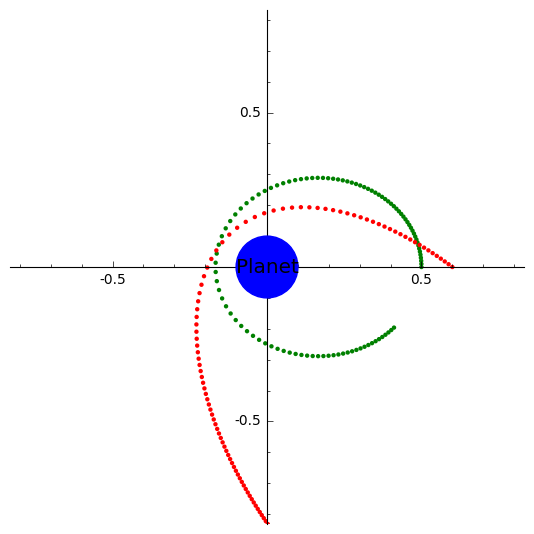
\includegraphics[scale=0.60]{figures/part0.png}
\end{figure}
%
Make sure you understand what each argument of orbit\_plot() means;
Refer to the table below:
\begin{enumerate}
  \item $x_i$ of the satellite ($y_i = 0$ by default)
  \item $v_{xi}$ of the satellite
  \item $v_{yi}$ of the satellite
  \item the gravitational force law, i.e. $F_g = 1/r^2$ (see above)
  \item the time interval between data points, make this smaller for more detail
  \item the path length at which the calculations stops, make this larger to see more of the path
  \item the color of the data points
\end{enumerate}
Adjust a few settings to see how they affect your resulting plot.
\hfill \break

\underline{\textbf{Part 1}} \par
Create two circular orbits of different radii.
Record your initial values and a screenshot of your plot.
%
\begin{figure}[H]
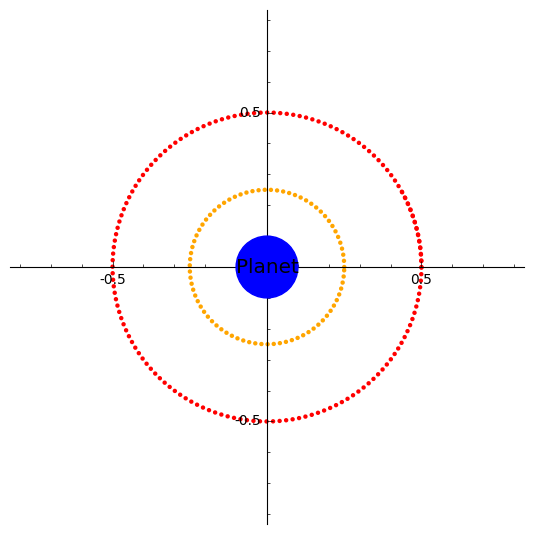
\includegraphics[scale=0.60]{figures/part1.png}
\end{figure}

\underline{\textbf{Part 2}} \par
a) Create an elliptical orbit by either
\begin{itemize}
\item making the velocity too large
\item making the velocity too small
\item making the velocity non-tangent to a circular path.
\end{itemize}
b) Create a case where the velocity is larger than the escape velocity.

Record your conditions and a screenshot of your plot.
%
\begin{figure}[H]
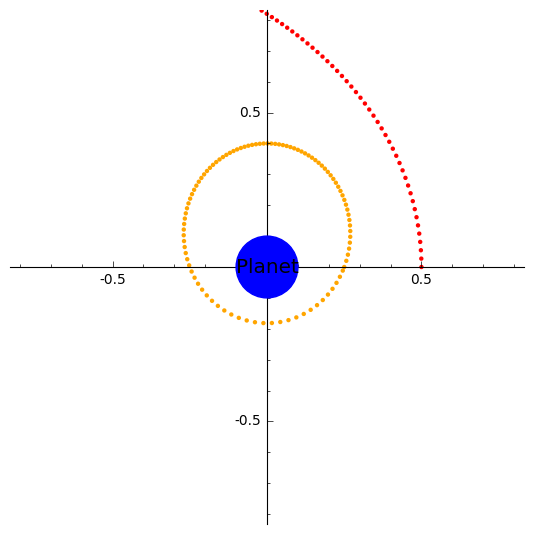
\includegraphics[scale=0.60]{figures/part2.png}
\end{figure}

\underline{\textbf{Part 3}} \par
Design your own universe with a different gravitational force law.
Experiment until you find an interesting result.
Record your conditions and a screenshot of your plot.
%
\begin{figure}[H]
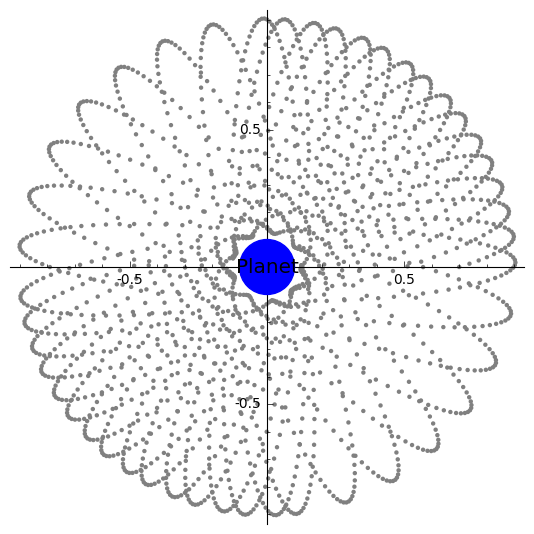
\includegraphics[scale=0.60]{figures/part3.png}
\end{figure}



\end{document}
